% !TeX encoding=utf8
% !TeX spellcheck = de-CH

%%% --- title based on maketitle --- --- --- ---

% \subject{Master thesis \\ University <insert>}
% \title{<insert title>}
% \author{<insert author>}
% \date{<insert date>}
% \maketitle


%%% --- title for this template --- --- --- ---

\begin{titlepage}
	\mbox{}\vspace{5\baselineskip}\\
	\rmfamily\huge
	\centering
	% \textsc{EVALUIERUNG DER RETRIEVAL-LEISTUNG EINER SEARCH ENGINE AM BEISPIEL DER BIBEL} \\
	\textsc{Evaluierung der Retrieval-Leistung einer Search Engine am Beispiel der Bibel} \\
	
	% \mbox{}\vspace{1\baselineskip}\\
	\vspace{2em}
	Michael Hadorn\\
	\vspace{\baselineskip}
	\rmfamily\Large
	\today\\
	Version \input{version.txt}\mbox{} \\
	\normalsize
	
	\vspace{6em}
	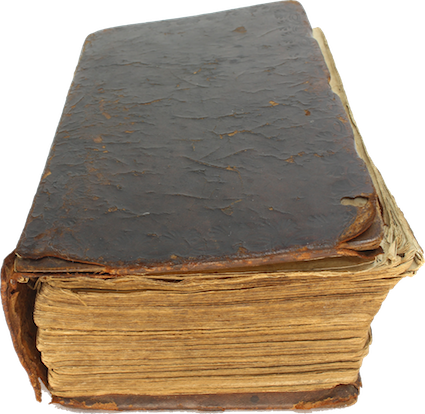
\includegraphics[width=0.3\textwidth]{images/0-title/bible.png}
	
	\vfill

	\begin{center}
		\begin{tabular}[h]{ r l }
			\textsc{\small{Studiengang}} & Informatik 8 BA 2012\\
			\textsc{\small{Seminararbeit}} & 2016\\
			\textsc{\small{Dozentin}} & Dr. Ruxandra Domenig\\
			\textsc{\small{Schule}} & ZHAW - School of Engineering\\
		\end{tabular}
	\end{center}

\end{titlepage}

%\begin{titlepage}
%   \mbox{}\vspace{5\baselineskip}\\
%   \rmfamily\huge
%   \centering
%   % title
%   \textsc{Workstation in the Cloud} \\[2ex]
%   Seminar: Cloud als Geschäftsmodell
%   \rmfamily\Large\\
%   \vspace{1\baselineskip}
%   bei Christian Vils\\
%   \vspace{1\baselineskip}
%   \input{version.txt}\mbox{}
%%   \vspace{3\baselineskip}\\
%%   <insert institute/university>
%   \vspace{5\baselineskip}\\
%   \rmfamily\Large
%   Simon Lang, Michael Hadorn
%   \vspace{1\baselineskip}\\
%   \today
%\end{titlepage}
 

%%% --- title for bachelor / master thesis --- --- --- ---

% \begin{titlepage}
% 	\mbox{}\vspace{5\baselineskip}\\
% 	\sffamily\huge
% 	\centering
% 	<insert title>
% 	\vspace{3\baselineskip}\\
% 	\rmfamily\Large
% 	Master thesis \\ University <insert>
% 	\vspace{2\baselineskip}\\
% 	\rmfamily\Large
% 	<insert author>
% 	\vspace{1\baselineskip}\\
% 	<insert date>
% \end{titlepage}

%%% --- title for phd thesis --- --- --- ---
% 
% -> check your faculty documents, this is 
%    usually stipulated
